%%%%%%%%%%%%%%%%%%%%%%%%%%%%%%%%%%%%%%%%%
% University Assignment Title Page 
% LaTeX Template
% Version 1.0 (27/12/12)
%
% This template has been downloaded from:
% http://www.LaTeXTemplates.com
%
% Original author:
% WikiBooks (http://en.wikibooks.org/wiki/LaTeX/Title_Creation)
%
% License:
% CC BY-NC-SA 3.0 (http://creativecommons.org/licenses/by-nc-sa/3.0/)
% 
% Instructions for using this template:
% This title page is capable of being compiled as is. This is not useful for 
% including it in another document. To do this, you have two options: 
%
% 1) Copy/paste everything between \begin{document} and \end{document} 
% starting at \begin{titlepage} and paste this into another LaTeX file where you 
% want your title page.
% OR
% 2) Remove everything outside the \begin{titlepage} and \end{titlepage} and 
% move this file to the same directory as the LaTeX file you wish to add it to. 
% Then add \input{./title_page_1.tex} to your LaTeX file where you want your
% title page.
%
%%%%%%%%%%%%%%%%%%%%%%%%%%%%%%%%%%%%%%%%%
%\title{Title page with logo}
%----------------------------------------------------------------------------------------
%	PACKAGES AND OTHER DOCUMENT CONFIGURATIONS
%----------------------------------------------------------------------------------------

\documentclass[12pt]{article}
\usepackage[english]{babel}
\usepackage[utf8x]{inputenc}
\usepackage{amsmath}
\usepackage{graphicx}
\usepackage{caption}
\usepackage{hyperref} 
\usepackage[colorinlistoftodos]{todonotes}
\setlength{\parskip}{1em}

\begin{document}

\begin{titlepage}

\newcommand{\HRule}{\rule{\linewidth}{0.5mm}} % Defines a new command for the horizontal lines, change thickness here

\center % Center everything on the page
 
%----------------------------------------------------------------------------------------
%	HEADING SECTIONS
%----------------------------------------------------------------------------------------

\textsc{\LARGE Ukrainian Catholic University}\\[1cm] % Name of your university/college
\textsc{\Large Applied Sciences Faculty}\\[0.5cm] % Major heading such as course name
\textsc{\large Data Science Master Programme}\\[0.5cm] % Minor heading such as course title

%----------------------------------------------------------------------------------------
%	TITLE SECTION
%----------------------------------------------------------------------------------------

\HRule \\[0.4cm]
{ \huge \bfseries SVD}\\[10pt]
{\Large \bfseries Project report}\\[0.4cm] % Title of your document
\HRule \\[1cm]
 
%----------------------------------------------------------------------------------------
%	AUTHOR SECTION
%----------------------------------------------------------------------------------------


% If you don't want a supervisor, uncomment the two lines below and remove the section above
\Large \emph{Authors:}\\
Yuriy Pryyma \\
Yuriy Kaminskyi\\[1cm] % Your name

%----------------------------------------------------------------------------------------
%	DATE SECTION
%----------------------------------------------------------------------------------------

{\large \today}\\[2cm] % Date, change the \today to a set date if you want to be precise

%----------------------------------------------------------------------------------------
%	LOGO SECTION
%----------------------------------------------------------------------------------------


\includegraphics[height=4cm]{UCU-Apps.png}\\[1cm] % Include a department/university logo - this will require the graphicx package
 
%----------------------------------------------------------------------------------------

\vfill % Fill the rest of the page with whitespace

\end{titlepage}


\begin{abstract}
This paper implements a real-time system to
recognize faces. The approach is essentially
to apply the concepts of vector space and
subspace to face recognition. The set of
known faces with m × n pixels forms a
subspace, called “face space”, of the “image
space” containing all images with m × n
pixels. This face space best defines the
variation of the known faces. The basis of
the face space is defined by the singularvectors
of the set of known faces. These
singular-vectors do not necessarily correspond
to the distinct features like ears,
eyes and noses. The projection of a new
image onto this face space is then compared
to the available projections of known faces
to identify the person. Since the dimension
of face subspace is much less than the whole
image space, it is much easier to compare
projections than origin images pixel by pixel.
Based on the above idea, a Singular Value
Decomposition (SVD) approach is
implemented in this paper. The framework
provides our system the ability to learn to
recognize new faces in a real-time and
automatic manner.
\end{abstract}

\section{Introduction}

SVD is a powerful tool in digital signal and image processing. It states that a
matrix can be decomposed as follows,
\begin{equation}
A=U \Sigma V^T
\end{equation}
Where $A_{m×n}$ is a dense matrix, $U_{m×m}$ and $V_{n×n}$ are orthogonal (or unitary) matrices and their columns are called left and right singular vectors respectively.
$\Sigma$ is a diagonal matrix and contains all singular values along its diagonal in a
non-increasing order. For a symmetric matrix m = n and U and V span the
same vector space. Hence computation of either U or V is sufficient. For any
dense symmetric matrix An×n, Eigen Value Decomposition (EVD) is defined as
follows
\begin{equation}
X=X \Lambda X^T
\end{equation}
Where X is the matrix of eigenvectors and $\Lambda$ is the diagonal matrix containing
eigenvalues along its diagonal. For symmetric matrices, eigenvalue decompositions
and singular value decompositions are closely related as follows [5]:
Suppose that $A$ is a symmetric matrix, with eigenvalues $\Lambda_i$ and orthonormal
eigen vectors ui so that $A=U \Lambda U^T$
is an eigenvalue decomposition of $A$, with
$/Lambda = diag[ \lambda{_1} \lambda{_2}...\lambda{_n}]$, $U = [u_1 u_2...u_n]$ and $UU^T = I$. Then an SVD of symmetric
matrix $A$ is, $A = U \Sigma V^T$
, where diagonal elements of $\Sigma$ i.e. $\sigma_i = abs(\lambda_i)$ and
$v_i = sign(\sigma_i).u_i$ where $sign(0) = 1$. For symmetric positive definite matrices
eigenvalue decomposition (EVD) and SVD leads to the same decomposition.
Hence we will use eigenvalues/eigenvectors and singular values/singular vectors
interchangeably.\par
However, SVD has been an offline tool for digital signal and image processing
applications for decades because of the computation complexity and memory
requirement. Due to the increased resources of some of the recently introduced
workstations, there are attempts to develop faster versions of SVD algorithm
for real-time signal and image processing applications. The implementation of
SVD in embedded platforms like DSPs, ARM and FPGAs is necessary for facilitating
efficient real-time image processing. Most of these platforms either have
fixed-point processors or CLBs (Configurable Logic Blocks) to make the system
cheaper and power efficient. Hence fast and fixed-point SVD algorithms are to
be developed for such applications. The purpose of this work is to evaluate the
existing SVD algorithms for their suitability on embedded platforms.\par
In pattern recognition, eigenspace based method has been proposed for face
tracking or face recognition [1]-[4]. To find the eigenspace, SVD (or eigenvalue
decomposition) is used. There are several algorithms for SVD as stated in literature
[5]-[7]. Jacobi’s algorithm is known to be the oldest and slowest algorithm
[5]-[8].For symmetric matrices, though Jacobi’s algorithm generates accurate singular
values and singular vectors, the time of execution increases with the dimension
of the matrices and is only suitable as an offline tool.Two-sided and
one-sided variants for Jacobi’s algorithm are stated in literature. Hestenes’ algorithm
is a variant of one-sided Jacobi’s algorithm and is discussed in [9]-[10].
Being a one-sided version the time of computation is lesser than two-sided Jacobi’s
algorithm. However, as the iteration is applied on the whole process this
algorithm is also not suitable for online applications. Golub and Kahan proposed
a two-step algorithm [6],[11]-[12] for computation of SVD. In the first step, a
dense symmetric matrix is converted to a bidiagonal matrix, which is eventually
Fast SVD 3
converted to a diagonal matrix using implicit QR iteration in the second step.
Because the second phase of Golub-kahan algorithm is iterative in nature, it is
much faster than Jacobi’s or Hestenes’ algorithm. A similar two step algorithm
has been proposed for SVD, where a dense symmetric matrix is reduced to tridiagonal
matrix and then an implicit symmetric QR iteration is applied to reduce
the symmetric tridiagonal matrix into a diagonal matrix. This algorithm is found
to be faster and competitive with Golub-Kahan algorithm when a combination
of QR and QL algorithm is used [5]-[7]. Still these algorithms could not satisfy
real-time constraints as required by the signal and image processing platforms.
Hence a Divide and Conquer algorithm was proposed by J.J.M. Cuppen based on
a rank-one modification by Bunch, Nielsen and Sorensen. This is the fastest algorithm
till date when a complete eigensytem of a symmetric tridiagonal matrix is
required [5]. A variant of the said algorithm by Gu and Eisenstat has been implemented
in LAPACK routine for matrices with dimension larger than 25 [13]-[14].
Faster performance is achieved when floating-point SVD is converted to fixedpoint
format and implemented in fixed-point platform [22]. Fast and Fixed-point
SVD algorithm is also useful for reducing silicon area and power consumption
in embedded platforms [24]-[25]. For Digital Signal Processing applications, attempts
have been made to implement SVD algorithm using multiprocessor arrays
[26] and CORDIC (COordinate Rotation DIgital Computer) based reconfigurable
systems [27]-[28].\par
\par
\par
\section{SVD Approach for Face Recognition} 
Over the past decades, face image compression,
representation and recognition has drawn wide 
attention from researchers in  arrears of
computer  vision, neural network, pattern 
recognition, machine  learning, and so on. The 
application of face recognition includes: 
Access Control based  on the  face recognition, Computer  ­human interaction, Information 
Security, Law enforcement, Smart Car etc. [11]\par
Several approaches to face  recognition have 
been proposed  for the  2­dimensional facial 
recognition. Much of the work has focused on 
detecting individual features such as eyes, nose, 
mouth, and  head  outline,  and  defining  a  face 
model by the  position, size,  and  relationships
among these features [12][13].
\par
SVD  approach treats a set  of known faces as
vectors in a  subspace,  called  “face  space”, spanned by a small group of “base­faces”[1]. It 
likes Principal Component Analysis (PCA) [14],
recognition is performed  by projecting  a  new 
image onto the face space, and then classifying 
the face by comparing its coordinates (position)
in face space with the coordinates (positions) of
known faces. However, the SVD approach has
better numerical properties than PCA.\par
In this case, we redefined the matrix A as set of
the training face. Assume  each face  image has
m × n = M pixels, and is represented as an M × 
1  column  vector $f_i$ , a  ‘training  set’ S with N
number  of face  images of known individuals
forms an M × N matrix: 
\[
S = [ f{_1} f{_2}...f{_N}]
\]
The mean image f of set S, is mean value through all subset.
Subtracting f from the original faces gives.
\[
a_i = f_i  - f,        i = 1, 2,... N
\]
This gives another M × N matrix A: 
\[
A = [ a{_1} a{_2}...a{_N}]
\]
Since $\{ u_1, u_2,  u_r\}$ form an orthonormal basis
for R(A), the range (column) subspace of matrix
A. Since matrix A is formed from a training set
S with N face  images, R(A) is called  a  ‘face 
subspace’ in the ‘image space’ of m × n pixels, and each $u_i$ , i = 1,2 ,...,r , can be called a ‘base­ 
face’.\par
Let $x =[x_1, x_2,..., x_r ]^T$ be  the  coordinates
(position) of any m × n face image f in the face 
subspace. Then it is the  scalar  projection of
$f - \b f$ onto the base­faces:
$x = [u_1, u_2,...,u_r]^T(f - \b f)$ (21)
This coordinate  vector x is used to find which 
of the training faces best describes the 
face  f. That is to  find  some  training  face $f_i$ ,
i = 1,2 ,...,N , that minimizes the distance:
$ e_i= [(x - x_i)^T(x - x_i)]^{1/2}$
where $x_i$ is the coordinate vector of
$f_i$ , which is
the  scalar  projection of $f - f_i$ onto  the  base­ 
faces:$x_i = [u_1, u_2,..., u_r]^T(f_i - f)$
A face f is classified  as face $f_i$ when the 
minimum $e_i$ is less than some  predefined
threshold  $e_0$ . Otherwise  the  face  f is classified 
as “unknown face”.
If f is not  a  face, its distance  to the  face 
subspace will be greater than 0. Since the vector
projection of f - f onto the face space is given 
by$f_p = [ u_1, u_2,..., u_r ]x$
The  distance  of f to the  face  space  is the 
distance  between f - f and  the  projection $f_p$
onto the face space.
If $e_f$ is greater than some predefined threshold 
$e_1$ , then f is not a face image.

\section{Steps to Conduct FR with SVD}
The steps for face recognition with SVD are the following:\par
1. Obtain a  training  set S with N face 
images of known individuals.\par
\begin{center}  
	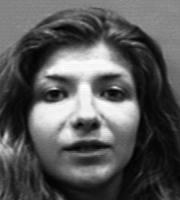
\includegraphics[height=5cm]{dataset_img.jpg}
	\captionof{figure}{Gray scale training set image}
\end{center}
2. Compute the mean face f of S.\par
\begin{center}  
	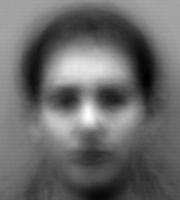
\includegraphics[height=4cm]{mean_img.jpg}
	\captionof{figure}{Mean image}
\end{center}
3. Forms a  matrix A with the 
computed f .\par
\begin{center}  
	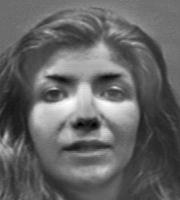
\includegraphics[height=4cm]{diff_img.jpg}
	\captionof{figure}{Diff of face image and mean image}
\end{center}
4. Calculate the SVD of A\par
5. For each known individual, compute the 
coordinate vector $x_i$. Choose a 
threshold $e_1$ that  defines the  maximum 
allowable  distance from face  space. Determine  a  threshold  $e_0$ that defines
the  maximum allowable  distance  from 
any known face in the training set S.\par
6. For a new input image f to be identified, 
calculate  its coordinate  vector x, the  vector projection $f_p$ , the 
distance $e_f$ to the face space.
If $e_f$ >  $e_1$ the input image is not a face. \par
7. If $e_f$ <  $e_1$, compute  the  distance $e_i$ to 
each known individual. If all $e_i >  e_0$ ,
the  input  image may be  classified  as
unknown face,  and  optionally used  to 
begin a new individual face. If $e_f$ <  $e_1$,
and  some $e_i <  e_0$ , classify the  input 
image as the  known individual 
associated  with the  minimum $e_i$ ($x_i$),
and this image may optionally added to 
the  original training set. Steps 1­-5 may 
be repeated. This can update the system with more instances of known faces.
\section{Experiments and results}
We implemented algorim in jupyter notebook[31].
For algorim testing we have used Face94 dataset[32] \\
Database Description:\par
1. Number of individuals: 153\par
2. Image resolution: 180 by 200 pixels (portrait format)\par
3. Directories: female (20), male (113), malestaff(20)\par
4. Contains images of male and female subjects in separate directories\par
For algorims accuracy extimation was used 153 train face images(for each individual) and 500 test images randomly chosen from the rest of the dataset. \\
	Resulted algorithms accuracy is 93.5\%.
\section{References}
1. Yang M-H., Kriegman D. J. and Ahuja N.: Detecting Faces in Images: A Survey”,
IEEE Transactions on Pattern Analysis and Machine Intelligence, Vol. 24, No. 1,
Fast SVD 19
January 2001.\par
2. Hjelms E. and Low B. K.: Face Detection: A Survey, Computer Vision and Image
Understanding 83, 236-274 (2001).\par
3. Sirovich L. and Kirby M.: Low-dimensional Procedure for the Characterization of
Human Faces, Journal of the Optical Society of America A, Vol. 4, P 519, March
1987.\par
4. Turk M. and Pentland A.: Eigenfaces for Recognition, Journal of Cognitive Neuroscience
Volume 3, Number 1, 1991.\par
5. Demmel J. W.: Applied Numerical Linear Algebra, SIAM, Philadelphia, 1997.\par
6. Golub G. H. and Van Loan C. F.: Matrix Computations, Third Editions, The
Jhons Hopkins University Press, Baltimore and London, 1996.\par
7. Datta B. N.: Numerical Linear Algebra and Applications, Brooks/Cole Publishing
Company, CA, USA, 1995.\par
8. Parlett B. N.: The Symmetric Eigenvalue Problem, SIAM, Philadelphia, 1998.\par
9. Hestenes M. R.:Inversion of Matrices by Biorthogonalization and Related Results”,
SIAM, Vol. 6, No. 1,March 1958, pp. 51-90.\par
10. Svensson G.: A Block-Hestenes Method for the SVD, hem.passagen.se/-
gohel/num/hest.ps, September 1989.\par
11. Golub G. and Kahan W.: Calculating the Singular Values and Pseudo-Inverse of
a Matrix , J. SIAM Numer. Anal., Ser. B, Vol. 2, No. 2, 1965.\par
12. Demmel J., Kahan W.: Accurate Singular Values of Bidiagonal Matrices, SIAM J.
Sci. Stat. Comput., v. 11, n. 5, pp. 873-912, 1990.\par
13. Bunch J. R., Nielsen C. P. and Sorensen D. C.: Rank-One Modification of the
Symmetric Eigenproblem, Numer. Math,31,31-48(1978).\par
14. Cuppen J.J.M.: A Divide and Conquer Method for the Symmetric Tridiagonal
Eigenproblem”, Numer. Math. 36, 177-195(1981).\par
15. Zhou B. B. and Brent R. P.: On Parallel Implementation of the
One-sided Jacobi Algorithm for Singular Value Decompositions”.\par
16. Stewart G. W.: Perturbation Theory for the Singular Value Decomposition”,
UMIACS-TR-90-124, CS-TR 2539, September 1990.\par
17. Gu M. and Eisenstat S.C.: A Divide-and-Conquer Algorithm For The Symmetric
Tridiagonal Eigen Problem, Research Report YALEU/DCS/RR-932, 27 November
1992.\par
18. Li R. C.: Solving Secular Equations Stably and Efficiently, Computer Science Division
Technical Report UCB//CSD-94-851, University of California, Berkeley, CA
94720, December, 1994.\par
19. Melman A.: A numerical comparison of methods for solving secular equations,
Jour. of Comp. and App. Math. 86(1997) 237-249.\par
20. Rutter J.: A Serial Implementation of Cuppen’s Divide
and Conquer Algorithm for the Symmetric Eigenvalue
Problem.http://www.netlib.org/lapack/lawnspdf/lawn69.pdf.\par
21. Anderson E., Bai Z., Bischof C., Blackford S., Demmel J., Dongarra J., Du Croz
J., Greenbaum A., Hammarling S., McKenney A., Sorensen D.: LAPACK Users’
Guide, Third Edition, 22 Aug, 1999.\par
22. Nikoli´c Z., Nguyen H. T., Frantz G.: Design and Implementation of Numerical
Linear Algebra Algorithms on Fixed Point DSPs, EURASIP Journal on Advances
in Signal Processing, Vol. 2007, Article ID 87046, doi: 10.1155/2007/87046.\par
23. Cilio A. G. M., and Corporaal H.: Floating point to fixed point conversion of C
code, Proceedings of CC 99, the 8th International Conference on Compiler Construction
(Lecture notes in computer science 1575), March 1999.\par
24. Kim S., Kum K., and Sung W.: Fixed-Point Optimization Utility for C and C++
Based Digital Signal Processing Programs, IEEE Transaction on Circuits and Systems
II: Analog and Digital Signal Processing, pp. 1455–1464, vol. 45, no. 11, Nov
1998.\par
25. Keding H., Willems M., Coors M., and Meyr H.: FRIDGE: A fixed-point design
and simulation environment, in Proc. Design Automation and Test in Europe,
1998, pp. 429–435.\par
26. Brent R. and Luk F.: The solution of singular value and symmetric eigenvalue
problems on multiprocessor arrays, SIAM J. Sci. Stat. Comput., 6, 1985, pp. 69-
84.\par
27. Wang H., Leray P., Palicot J.: A CORDIC-based dynamically reconfigurable FPGA
architecture for signal processing algorithms, URSI 08, The XXIX General Assembly
of the International Union of Radio Science, Chicago IL, 2008.\par
28. Szec´owka P. M. and Malinowski P.,: CORDIC and SVD Implementation in Digital
Hardware, MIXDES 2010, 17th International Conference ”Mixed Design of
Integrated Circuits and Systems”, june 24-26, 2010.\par
29. Dinges, D.F., Mallis, M., Maislin, G., Powell, J.W., 1998. Final Report: Evaluation
of Techniques for Ocular Measurement as an Index of Fatigue and as the Basis for
Alertness Management (Report No. DOT HS 808 762). National Highway Traffic
Safety Administration, Washington, DC.\par
30. Dinges, D.F., Maislin, G., Brewster, R.M., Krueger, G.P., Carroll, R.J., 2004. Pilot
Test of Fatigue Management Technologies: Final Report. Federal Motor Carrier
Safety Administration, Washington, DC.\par
31. \href{https://github.com/Houd1ny/SVDFaceRecognition}{SVDFaceRecognition source code}. \par
32. \href{http://cswww.essex.ac.uk/mv/allfaces/faces94.html}{Faces databes "faces94" }. \par

\end{document}